%!TEX root = ../artigo.tex
\section{Resultados}
A rede neural auto-organizável implementada nesse trabalho, utilizou o algoritmo Mapa de Kohonen, desenvolvido por
Teuvo Kohonen em 1982 \cite{Kohonen}. A implementação deste trabalho pode ser vista em \url{https://github.com/QSF/ia-kohonen}.

Para os resultados práticos, a rede foi treinada com um conjunto de 1728 exemplos de dados reais, fornecidos pelo site \textit{UCI Machine Learning Repository}\footnote{http://archive.ics.uci.edu/ml/}, variando valores da taxa de aprendizado, pesos iniciais, raio da vizinhança e quantidade de neurônios na rede. O conjunto de exemplos escolhido foi o \textit{Car Evaluation}\footnote{http://archive.ics.uci.edu/ml/datasets/Car+Evaluation}, onde dados os atributos preço de compra do veículo, custo da manutenção, quantidade de portas do veículo, número de passageiros, tamanho do bagageiro e segurança estimada do veículo, avalia se o veículo é aceitável, inaceitável, bom ou muito bom.

Uma vez que o algoritmo Mapa de Kohonen organiza ou agrupa dimensionalmente os dados, o conjunto de exemplos foi adaptado, apresentando somente três dimensões (preço de compra do veículo, custo da manutenção e segurança estimada do veículo). O primeiro e segundo atributo aceitos os valores {low, med, high e vhigh}, enquanto que o útilo aceita os valores {low, med, high}.

Com o conjunto de dados coletados, algumas entradas foram testadas para verificar a modificação final da rede. Esses testes serão exibidos a seguir, sendo dividido pela quantidade de neurônios na camada de saída (16, 20, 25 e 36 neurônios).

\subsection{16 neurônios} % (fold)
\label{sub:16_neuronios}

\begin{figure}[ht!]
	\centering
	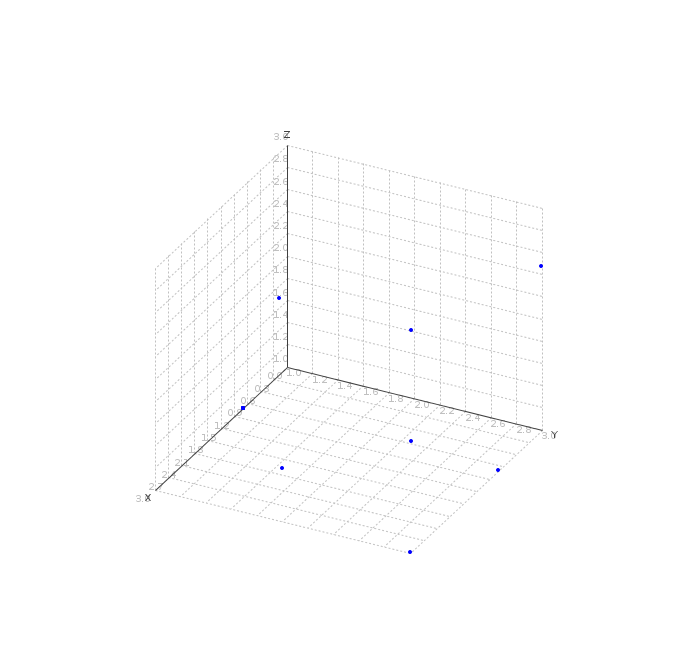
\includegraphics[scale=0.4]{./imgs/fig:out_16_teste_1}
	\caption{16 Neurônios - Teste 1}
	\label{fig:out_16_teste_1}
\end{figure}

\begin{figure}[ht!]
	\centering
	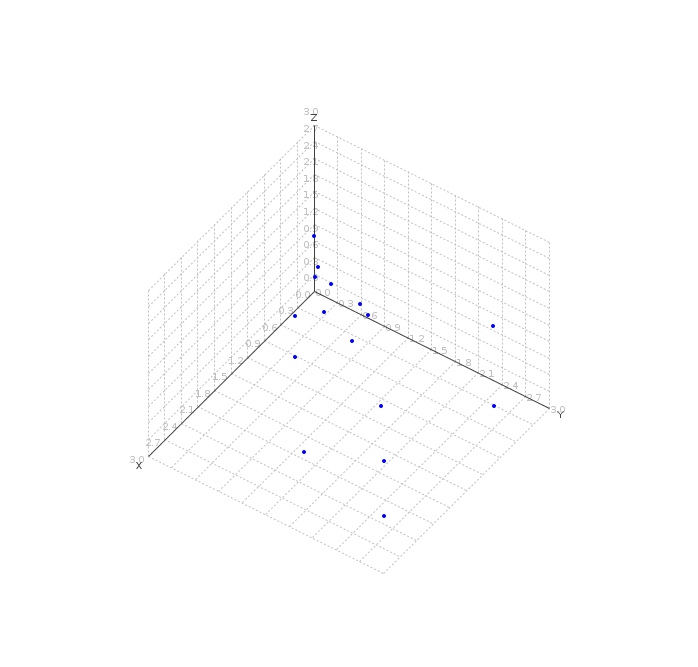
\includegraphics[scale=0.4]{./imgs/fig:out_16_teste_2}
	\caption{16 Neurônios - Teste 2}
	\label{fig:out_16_teste_2}
\end{figure}

\begin{figure}[ht!]
	\centering
	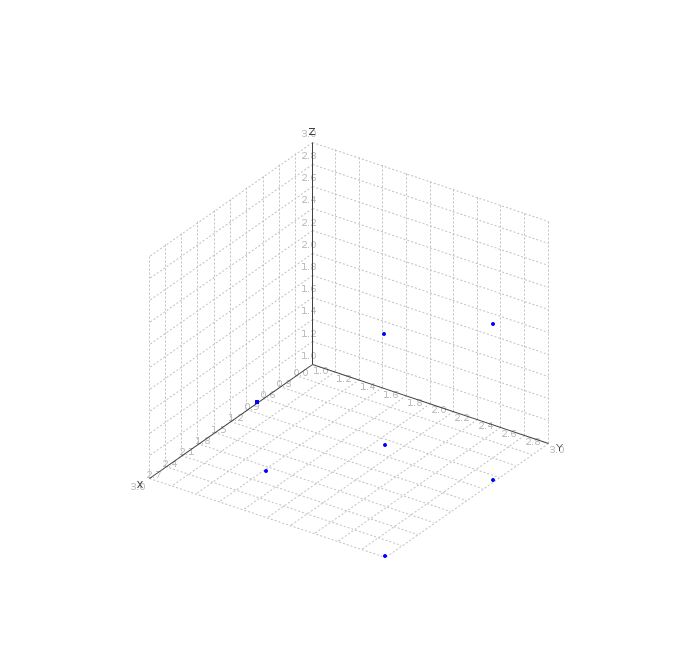
\includegraphics[scale=0.4]{./imgs/fig:out_16_teste_3}
	\caption{16 Neurônios - Teste 3}
	\label{fig:out_16_teste_3}
\end{figure}

\begin{figure}[ht!]
	\centering
	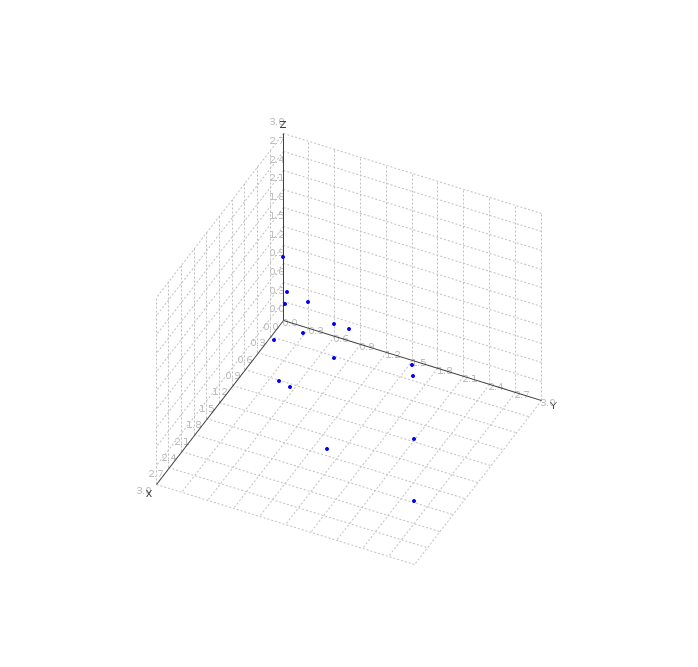
\includegraphics[scale=0.4]{./imgs/fig:out_16_teste_4}
	\caption{16 Neurônios - Teste 4}
	\label{fig:out_16_teste_4}
\end{figure}

Nos conjuntos de teste apresentados por essa seção, a rede possuia 16 neurônios na camada de saída, sendo que sua topologia é da forma de uma grade 4x4.

Para realizar os testes na rede mencionada, foi variado o valor da taxa de aprendizagem e dos pesos inicias, com raio fixo em 0.

Quatro testes foram executados, onde a configuração da rede para cada caso é ilustrada em ~\ref{table:dados_16}.
\begin{table}[ht]
\caption{Configurações da Rede com 16 Neurônios na Saída}
\centering
\begin{tabular}{|c|c|c|}  \hline
   Teste 	& Taxa de Aprendizagem 	& Pesos Inicias 	\\ \hline
   1 		& 0.1 				 	& todos 1 			\\ \hline
   2 		& 0.1 				 	& Random 			\\ \hline
   3 		& 0.3 				 	& todos 1 			\\ \hline
   4 		& 0.3 				 	& Random 			\\ \hline
\end{tabular}
\label{table:dados_16}
\end{table}

As figuras \ref{fig:out_16_teste_1}, \ref{fig:out_16_teste_2}, \ref{fig:out_16_teste_3} e \ref{fig:out_16_teste_4} representam a rede após a execução dos testes 1, 2, 3 e 4; respectivamente.

% subsection 16_neuronios (end)

\subsection{20 neurônios} % (fold)
\label{sub:20_neuronios}

\begin{figure}[ht!]
	\centering
	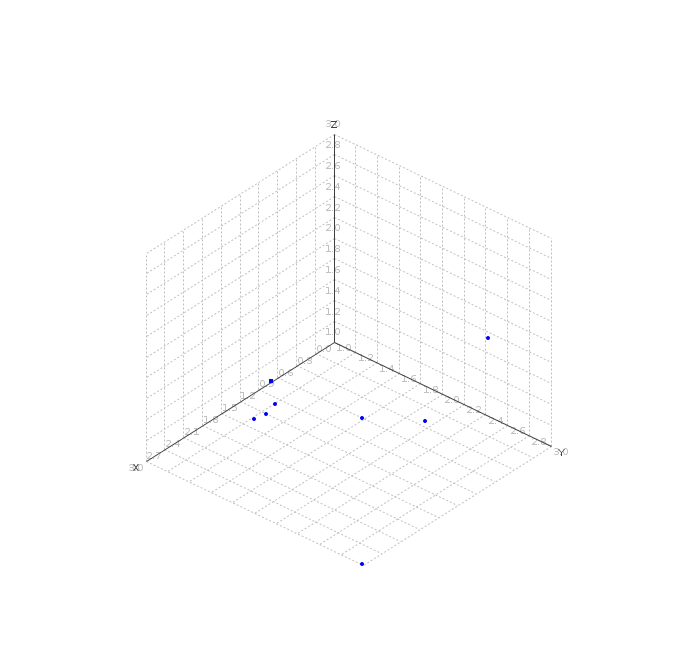
\includegraphics[scale=0.4]{./imgs/fig:out_20_teste_1}
	\caption{20 Neurônios - Teste 1}
	\label{fig:out_20_teste_1}
\end{figure}

\begin{figure}[ht!]
	\centering
	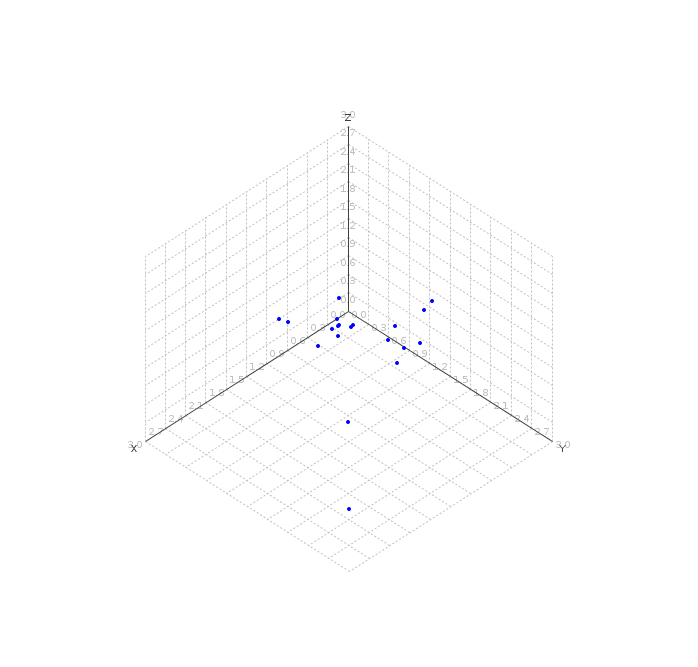
\includegraphics[scale=0.4]{./imgs/fig:out_20_teste_2}
	\caption{20 Neurônios - Teste 2}
	\label{fig:out_20_teste_2}
\end{figure}

\begin{figure}[ht!]
	\centering
	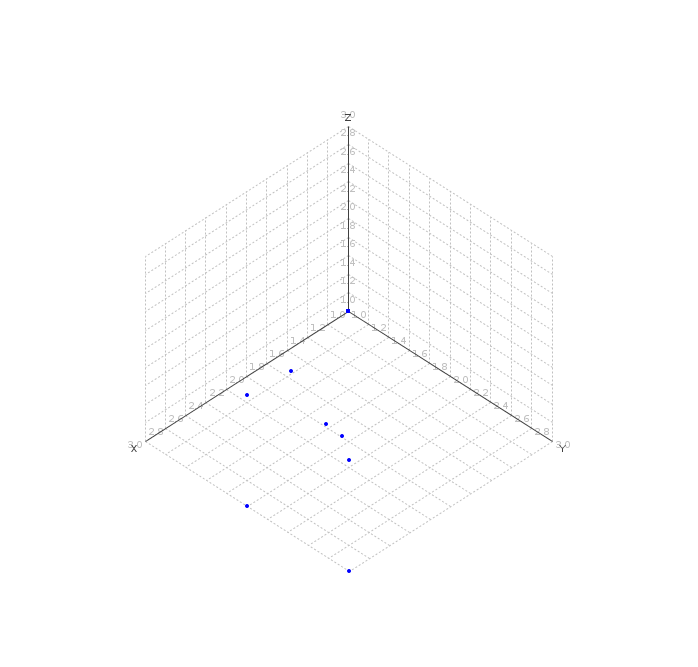
\includegraphics[scale=0.4]{./imgs/fig:out_20_teste_3}
	\caption{20 Neurônios - Teste 3}
	\label{fig:out_20_teste_3}
\end{figure}

\begin{figure}[ht!]
	\centering
	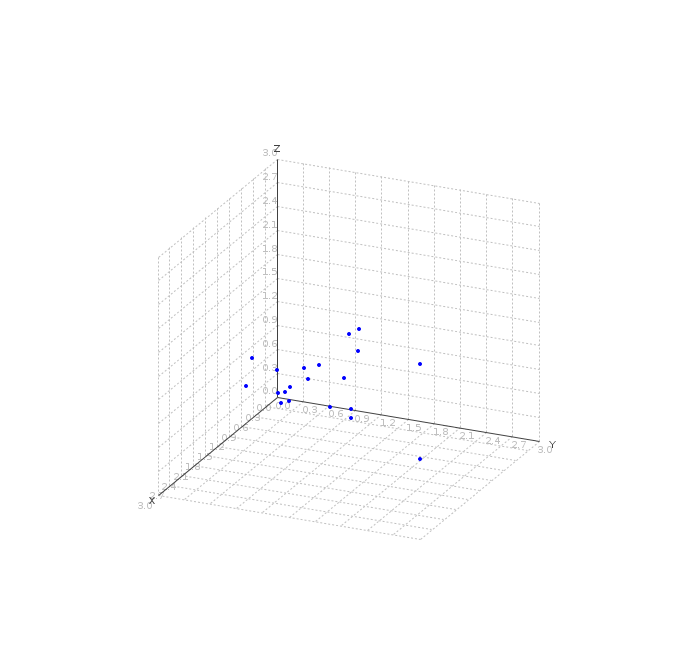
\includegraphics[scale=0.4]{./imgs/fig:out_20_teste_4}
	\caption{20 Neurônios - Teste 4}
	\label{fig:out_20_teste_4}
\end{figure}

Nesta seção, a rede possuia 20 neurônios na camada de saída, sendo uma grade 4x5.

Para realizar os testes na rede mencionada, novamente foi variado o valor da taxa de aprendizagem e dos pesos inicias, mas com raio fixo em 1.

Também foram executados quatro testes que tem sua configuração ilustrada na tabela ~\ref{table:dados_20}.
\begin{table}[ht]
\caption{Configurações da Rede com 20 Neurônios na Saída}
\centering
\begin{tabular}{|c|c|c|}  \hline
   Teste 	& Taxa de Aprendizagem 	& Pesos Inicias 	\\ \hline
   1 		& 0.5 				 	& todos 1 			\\ \hline
   2 		& 0.5				 	& Random 			\\ \hline
   3 		& 0.75 				 	& todos 1 			\\ \hline
   4 		& 0.75				 	& Random 			\\ \hline
\end{tabular}
\label{table:dados_20}
\end{table}

Os testes 1, 2, 3 e 4 são representados pelas imagens \ref{fig:out_20_teste_1}, \ref{fig:out_20_teste_2}, \ref{fig:out_20_teste_3} e \ref{fig:out_20_teste_4}; respectivamente.

% subsection 20_neuronios (end)

\subsection{25 neurônios}
Os gráficos a seguir mostram a plotação dos pontos após a execução do algoritmo para alguns valores de parâmetros e para 
uma rede com 25 neurônios. Apesar de não se poder afirmar se o algoritmo convergiu, vemos que aumentando o raio de vizinhança,
o algoritmo consegue ``especializar'' melhor o conjunto. O efeito da taxa de aprendizado está sobre a velocidade na qual o 
algoritmo irá convergir. Ela geralmente é dada empiricamente, assim como os pesos iniciais, que segundo \cite{Kohonen}, se forem
inicializados com valores iguais, faz o algoritmo convergir mais rapidamente.

\begin{figure}[ht!]
	\centering
	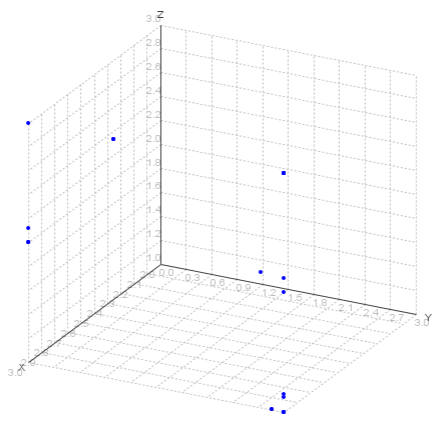
\includegraphics[scale=0.65]{./imgs/2a1.png}
	\caption{Taxa de aprendizado: 0.8662815917277779; Raio: 1; Pesos iniciais: A}
\end{figure}

\begin{figure}[ht!]
	\centering
	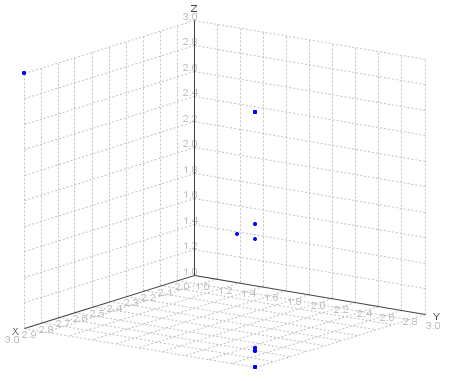
\includegraphics[scale=0.65]{./imgs/2a2.png}
	\caption{Taxa de aprendizado: 0.8662815917277779; Raio: 2; Pesos iniciais: A}
\end{figure}

\begin{figure}[ht!]
	\centering
	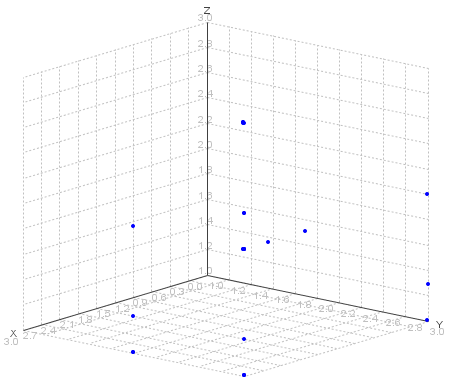
\includegraphics[scale=0.65]{./imgs/2b1.png}
	\caption{Taxa de aprendizado: 0.5980629675758204; Raio: 1; Pesos iniciais: B}
\end{figure}

\begin{figure}[ht!]
	\centering
	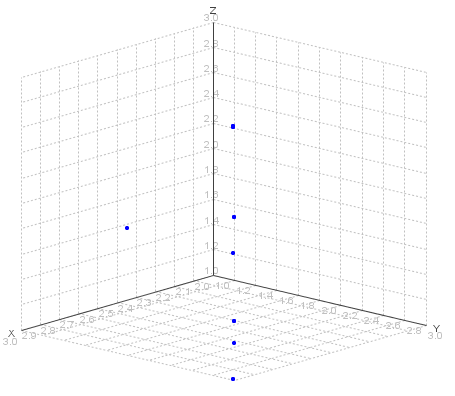
\includegraphics[scale=0.65]{./imgs/2b2.png}
	\caption{Taxa de aprendizado: 0.5980629675758204; Raio: 2; Pesos iniciais: B}
\end{figure}

\subsection{36 neurônios}
Os gráficos a seguir mostram a plotação dos pontos após a execução do algoritmo para alguns valores de parâmetros e para
uma rede com 36 neurônios.

\begin{figure}[ht!]
	\centering
	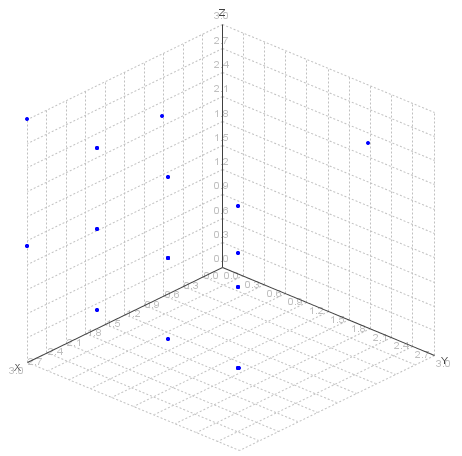
\includegraphics[scale=0.65]{./imgs/2d1.png}
	\caption{Taxa de aprendizado: 0.2625656059885696; Raio: 1; Pesos iniciais: D}
\end{figure}

\begin{figure}[ht!]
	\centering
	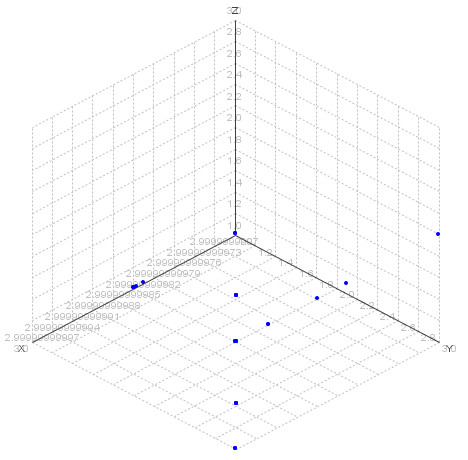
\includegraphics[scale=0.65]{./imgs/2d2.png}
	\caption{Taxa de aprendizado: 0.2625656059885696; Raio: 2; Pesos iniciais: D}
\end{figure}

\begin{figure}[ht!]
	\centering
	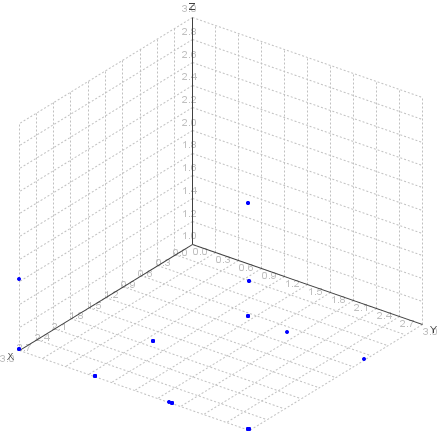
\includegraphics[scale=0.65]{./imgs/2e1.png}
	\caption{Taxa de aprendizado: 0.5517820314689292; Raio: 1; Pesos iniciais: E}
\end{figure}

\newpage
\begin{figure}[ht!]
	\centering
	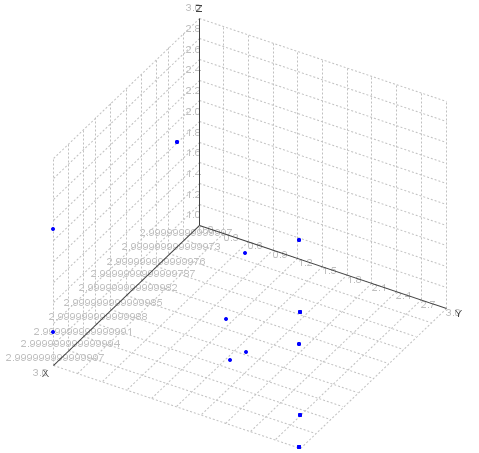
\includegraphics[scale=0.65]{./imgs/2e2.png}
	\caption{Taxa de aprendizado: 0.5517820314689292; Raio: 2; Pesos iniciais: E}
\end{figure}

